\documentclass[oneside,]{memoir}
\usepackage{amssymb,amsmath}
\usepackage{ifxetex,ifluatex}
\ifxetex
  \usepackage{fontspec,xltxtra,xunicode}
  \defaultfontfeatures{Mapping=tex-text,Scale=MatchLowercase}
  \newcommand{\euro}{€}
\else
  \ifluatex
    \usepackage{fontspec}
    \defaultfontfeatures{Mapping=tex-text,Scale=MatchLowercase}
    \newcommand{\euro}{€}
  \else
    \usepackage[utf8]{inputenc}
  \fi
\fi
% Redefine labelwidth for lists; otherwise, the enumerate package will cause
% markers to extend beyond the left margin.
\makeatletter\AtBeginDocument{%
  \renewcommand{\@listi}
    {\setlength{\labelwidth}{4em}}
}\makeatother
\usepackage{enumerate}
\usepackage{graphicx}
% We will generate all images so they have a width \maxwidth. This means
% that they will get their normal width if they fit onto the page, but
% are scaled down if they would overflow the margins.
\makeatletter
\def\maxwidth{\ifdim\Gin@nat@width>\linewidth\linewidth
\else\Gin@nat@width\fi}
\makeatother
\let\Oldincludegraphics\includegraphics
\renewcommand{\includegraphics}[1]{\Oldincludegraphics[width=\maxwidth]{#1}}
\ifxetex
  \usepackage[setpagesize=false, % page size defined by xetex
              unicode=false, % unicode breaks when used with xetex
              xetex,
              bookmarks=true,
              pdfauthor={},
              pdftitle={},
              colorlinks=true,
              linkcolor=blue]{hyperref}
\else
  \usepackage[unicode=true,
              bookmarks=true,
              pdfauthor={},
              pdftitle={},
              colorlinks=true,
              linkcolor=blue]{hyperref}
\fi
\hypersetup{breaklinks=true, pdfborder={0 0 0}}
\setlength{\parindent}{0pt}
\setlength{\parskip}{6pt plus 2pt minus 1pt}
\setlength{\emergencystretch}{3em}  % prevent overfull lines
\usepackage{fourier} % or what ever
\usepackage[scaled=.92]{helvet}%. Sans serif - Helvetica
\usepackage{color,calc}
\newsavebox{\ChpNumBox}
\definecolor{ChapBlue}{rgb}{0.00,0.65,0.65}
\definecolor{DarkBlue}{rgb}{0.00,0.20,0.65}
\definecolor{Black}{rgb}{0.00,0.00,0.00}
\makeatletter
\newcommand*{\thickhrulefill}{%
\leavevmode\leaders\hrule height 1\p@ \hfill \kern \z@}
\newcommand*\BuildChpNum[2]{%
\begin{tabular}[t]{@{}c@{}}
\makebox[0pt][c]{#1\strut} \\[.5ex]
\colorbox{ChapBlue}{%
\rule[-10em]{0pt}{0pt}%
\rule{1ex}{0pt}\color{black}#2\strut
\rule{1ex}{0pt}}%
\end{tabular}}
\makechapterstyle{BlueBox}{%
\renewcommand{\chapnamefont}{\large\scshape}
\renewcommand{\chapnumfont}{\Huge\bfseries}
\renewcommand{\chaptitlefont}{\raggedright\Huge\sffamily\bfseries}
\setlength{\beforechapskip}{20pt}
\setlength{\midchapskip}{26pt}
\setlength{\afterchapskip}{40pt}
\renewcommand{\printchaptername}{}
\renewcommand{\chapternamenum}{}
\renewcommand{\printchapternum}{%
\sbox{\ChpNumBox}{%
\BuildChpNum{\chapnamefont\@chapapp}%
{\chapnumfont\thechapter}}}
\renewcommand{\printchapternonum}{%
\sbox{\ChpNumBox}{%
\BuildChpNum{\chapnamefont\vphantom{\@chapapp}}%
{\chapnumfont\hphantom{\thechapter}}}}
\renewcommand{\afterchapternum}{}
\renewcommand{\printchaptertitle}[1]{%
\usebox{\ChpNumBox}\hfill
\parbox[t]{\hsize-\wd\ChpNumBox-1em}{%
\vspace{\midchapskip}%
\thickhrulefill\par
\chaptitlefont ##1\par}}%
}
\chapterstyle{BlueBox}
%\chapterstyle{dash}
%%% Creating an initial of the very first character of the content
\usepackage{lettrine}
\newcommand{\initial}[1]{
	\lettrine[lines=3,lhang=0.3,nindent=0em]{
		\color{ChapBlue}
		{\textsf{#1}}
	}{}
}

%%% Title, author and date metadata
\usepackage{titling} % For custom titles
\newcommand{\HorRule}{
	\color{DarkBlue} % Creating a horizontal rule
	\rule{\linewidth}{1pt}
}
\pretitle{
	\vspace{-30pt} \begin{flushleft} \HorRule 
	\fontsize{50}{50} \usefont{OT1}{phv}{b}{n} \color{ChapBlue} \selectfont 
}
\posttitle{\par\end{flushleft}\vskip 0.5em}

\preauthor{\begin{flushleft}\large \lineskip 0.5em \usefont{OT1}{phv}{b}{sl} \color{Black}}
\postauthor{\footnotesize \usefont{OT1}{phv}{m}{sl} \color{Black} 
	,\qquad % One could have the institution of author right here
	\par\end{flushleft}\HorRule
}
\newcommand{\modreq}{!}
\newcommand{\modquery}{?}
\newcommand{\modtrue}{\top}
\newcommand{\modfalse}{\bot}
\newcommand{\moderr}{\epsilon}
\newcommand{\modaux}{a}


\begin{document}

\chapter{pandocgen}

This is a generation framework for yielding PDF and HTML from good old
Markdown files. It uses the eminent
\href{http://johnmacfarlane.net/pandoc/}{Pandoc tool}, so the Markdown
files can use Pandoc extensions to provide a slicker output, including
mathematical expressions. For the pure Markdown syntax and its
semantics, there is a good introduction on
\href{http://daringfireball.net/projects/markdown/syntax/}{Daring
Fireball}.

\textbf{NOTE}: for some reason, the creator of Pandoc, John MacFarlane,
has not named the Pandoc Markdown extension language. I sometimes refer
to it as \textbf{PandocMarkdown}.

\textbf{NOTE}: Pandoc is capable of translating between a host of
formats, but this \textbf{pandocgen} project focuses on
(Pandoc-)Markdown input. See the graph at the bottom of this document
for all the various conversion options of Pandoc; it is quite
mind-blowing. The image is from the Pandoc site and is copyrighted by
John MacFarlane.

\section{Very, Very Quick Intro\ldots{}}

\begin{enumerate}[1.]
\item
  Add this project as a submodule

\begin{verbatim}
git submodule add git@github.com:davber/pandocgen.git
\end{verbatim}
\item
  Create some beautiful Markdown file, \texttt{MyCoolDoc.md}
\item
  Create a Makefile like this:

\begin{verbatim}
BASE=MyCoolDoc
include pandocgen/Makefile
\end{verbatim}
\item
  Make space for the generated files:

\begin{verbatim}
mkdir gen
\end{verbatim}
\item
  Create the PDF and HTML files:

\begin{verbatim}
make all
\end{verbatim}
\end{enumerate}
That is it! Now you have a PDF and HTML version of your Markdown
document.

For a quick generation, you can actually generate this README file ---
people always enjoy others eating their own dog food (or actually others
eating pet food in general\ldots{}) --- by

\begin{verbatim}
make --file sample.mk
\end{verbatim}
where \texttt{sample.mk} is this short make file

\begin{verbatim}
BASE=README
RES_OUT=rez/diagram.png
include Makefile
\end{verbatim}
This will generate output files in the \texttt{gen} directory. They are
also uploaded to this Wiki, as a \href{./gen/README.pdf}{PDF file} and
\href{./gen/README.html}{HTML file}.

\section{Dependencies}

There are some dependencies, though:

\begin{enumerate}[1.]
\item
  A Gnu \textbf{make} command, preferably version 3.80 or later. On most
  decent machines, this is already installed.
\item
  LaTex, such as \href{http://www.tug.org/texlive/}{TeX Live}.
\item
  \href{http://johnmacfarlane.net/pandoc/}{Pandoc} --- the tool actually
  doing the generation
\end{enumerate}
\section{Using It\ldots{}}

To use this framework, there are two paths:

\begin{enumerate}[1.]
\item
  Include the provided Makefile in your own Makefile, after a section
  where you specify a few custom parameters, as defined in the Custom
  Parameters section.
\item
  Set the custom parameters as environment variables and use the
  provided Makefile as is.
\end{enumerate}
\section{Building Targets}

All target versions of the Markdown document are generated in a
\texttt{gen} directory relative the current working directory. As a
convenience, this project contains such a directory in case you are
running \texttt{make} from there.

Each of the target formats has a corresponding make target, so you can
issue one of:

\begin{verbatim}
make pdf
make html
make tex
\end{verbatim}
There is also a universal target, which builds all formats:

\begin{verbatim}
make all
\end{verbatim}
\section{Customer Parameters}

These are the parameters you can set -- either via a initial section in
an embedding Makefile or as environment variables:

\begin{itemize}
\item
  \texttt{BASE} - that is the name of the Markdown document,
  \textbf{without} suffix, such as \texttt{MyCoolDoc}, which will then
  generate \texttt{MyCoolDoc.pdf}, \texttt{MyCoolDoc.html} and
  \texttt{MyCoolDoc.tex} in the \texttt{gen} directory.
  \textbf{MANDATORY}
\item
  \texttt{RES\_IN} - the input files for resources, such as images,
  needed by the document. This often includes Graphviz Dot files or
  other input formats for PDF- and PNG-based images. \textbf{OPTIONAL}
\item
  \texttt{RES\_OUT} - the corresponding generated resource files, which
  are often PDF and PNG files. \textbf{OPTIONAL}.
\item
  \texttt{RES\_GEN} - the full command to generate the \texttt{RES\_OUT}
  files from the \texttt{RES\_IN} files. \textbf{OPTIONAL}
\end{itemize}
\textbf{NOTE}: so there is only \textbf{one} mandatory parameter to set,
and that is \texttt{BASE}.

\textbf{NOTE}: the default behavior, described above, actually allows
you to include resources in an input-ready format, such as raw PNG and
PDF files, by merely setting the \texttt{RES\_OUT} to those files and
let the other two resource-related parameters be. That will translate
into a no-op for that make step.

\section{Helper Files}

The helper files reside in the \texttt{input} directory.

The helper files are:

\begin{itemize}
\item
  \texttt{my-template.latex} - this is the main template for LaTeX
  generation and, indirectly, for PDF generation. It uses some
  parameters that can be set from command line --- and is actually set
  by the provided Makefile --- such as \texttt{docuemntclass}, which the
  Makefile sets to \texttt{memoir}. See the Makefile for some of those
  parameters used.
\item
  \texttt{mytitle.tex} - this is the template for the title page, for
  LaTeX (and PDF\ldots{})
\item
  \texttt{mychapter.tex} - specifies the look of chapter headings for
  LaTeX (and PDF\ldots{})
\item
  \texttt{macros.tex} - some TeX macros. \textbf{NOTE} these macros are
  actually expanded by Pandoc itself in the case of non-TeX-based
  generation --- such as HTML --- so one can have shortcuts or other
  macros even for HTML.
\end{itemize}
\section{The Completely Connected World Of Pandoc}

Can you count the number of translations possible? \ldots{}

\begin{figure}[htbp]
\centering
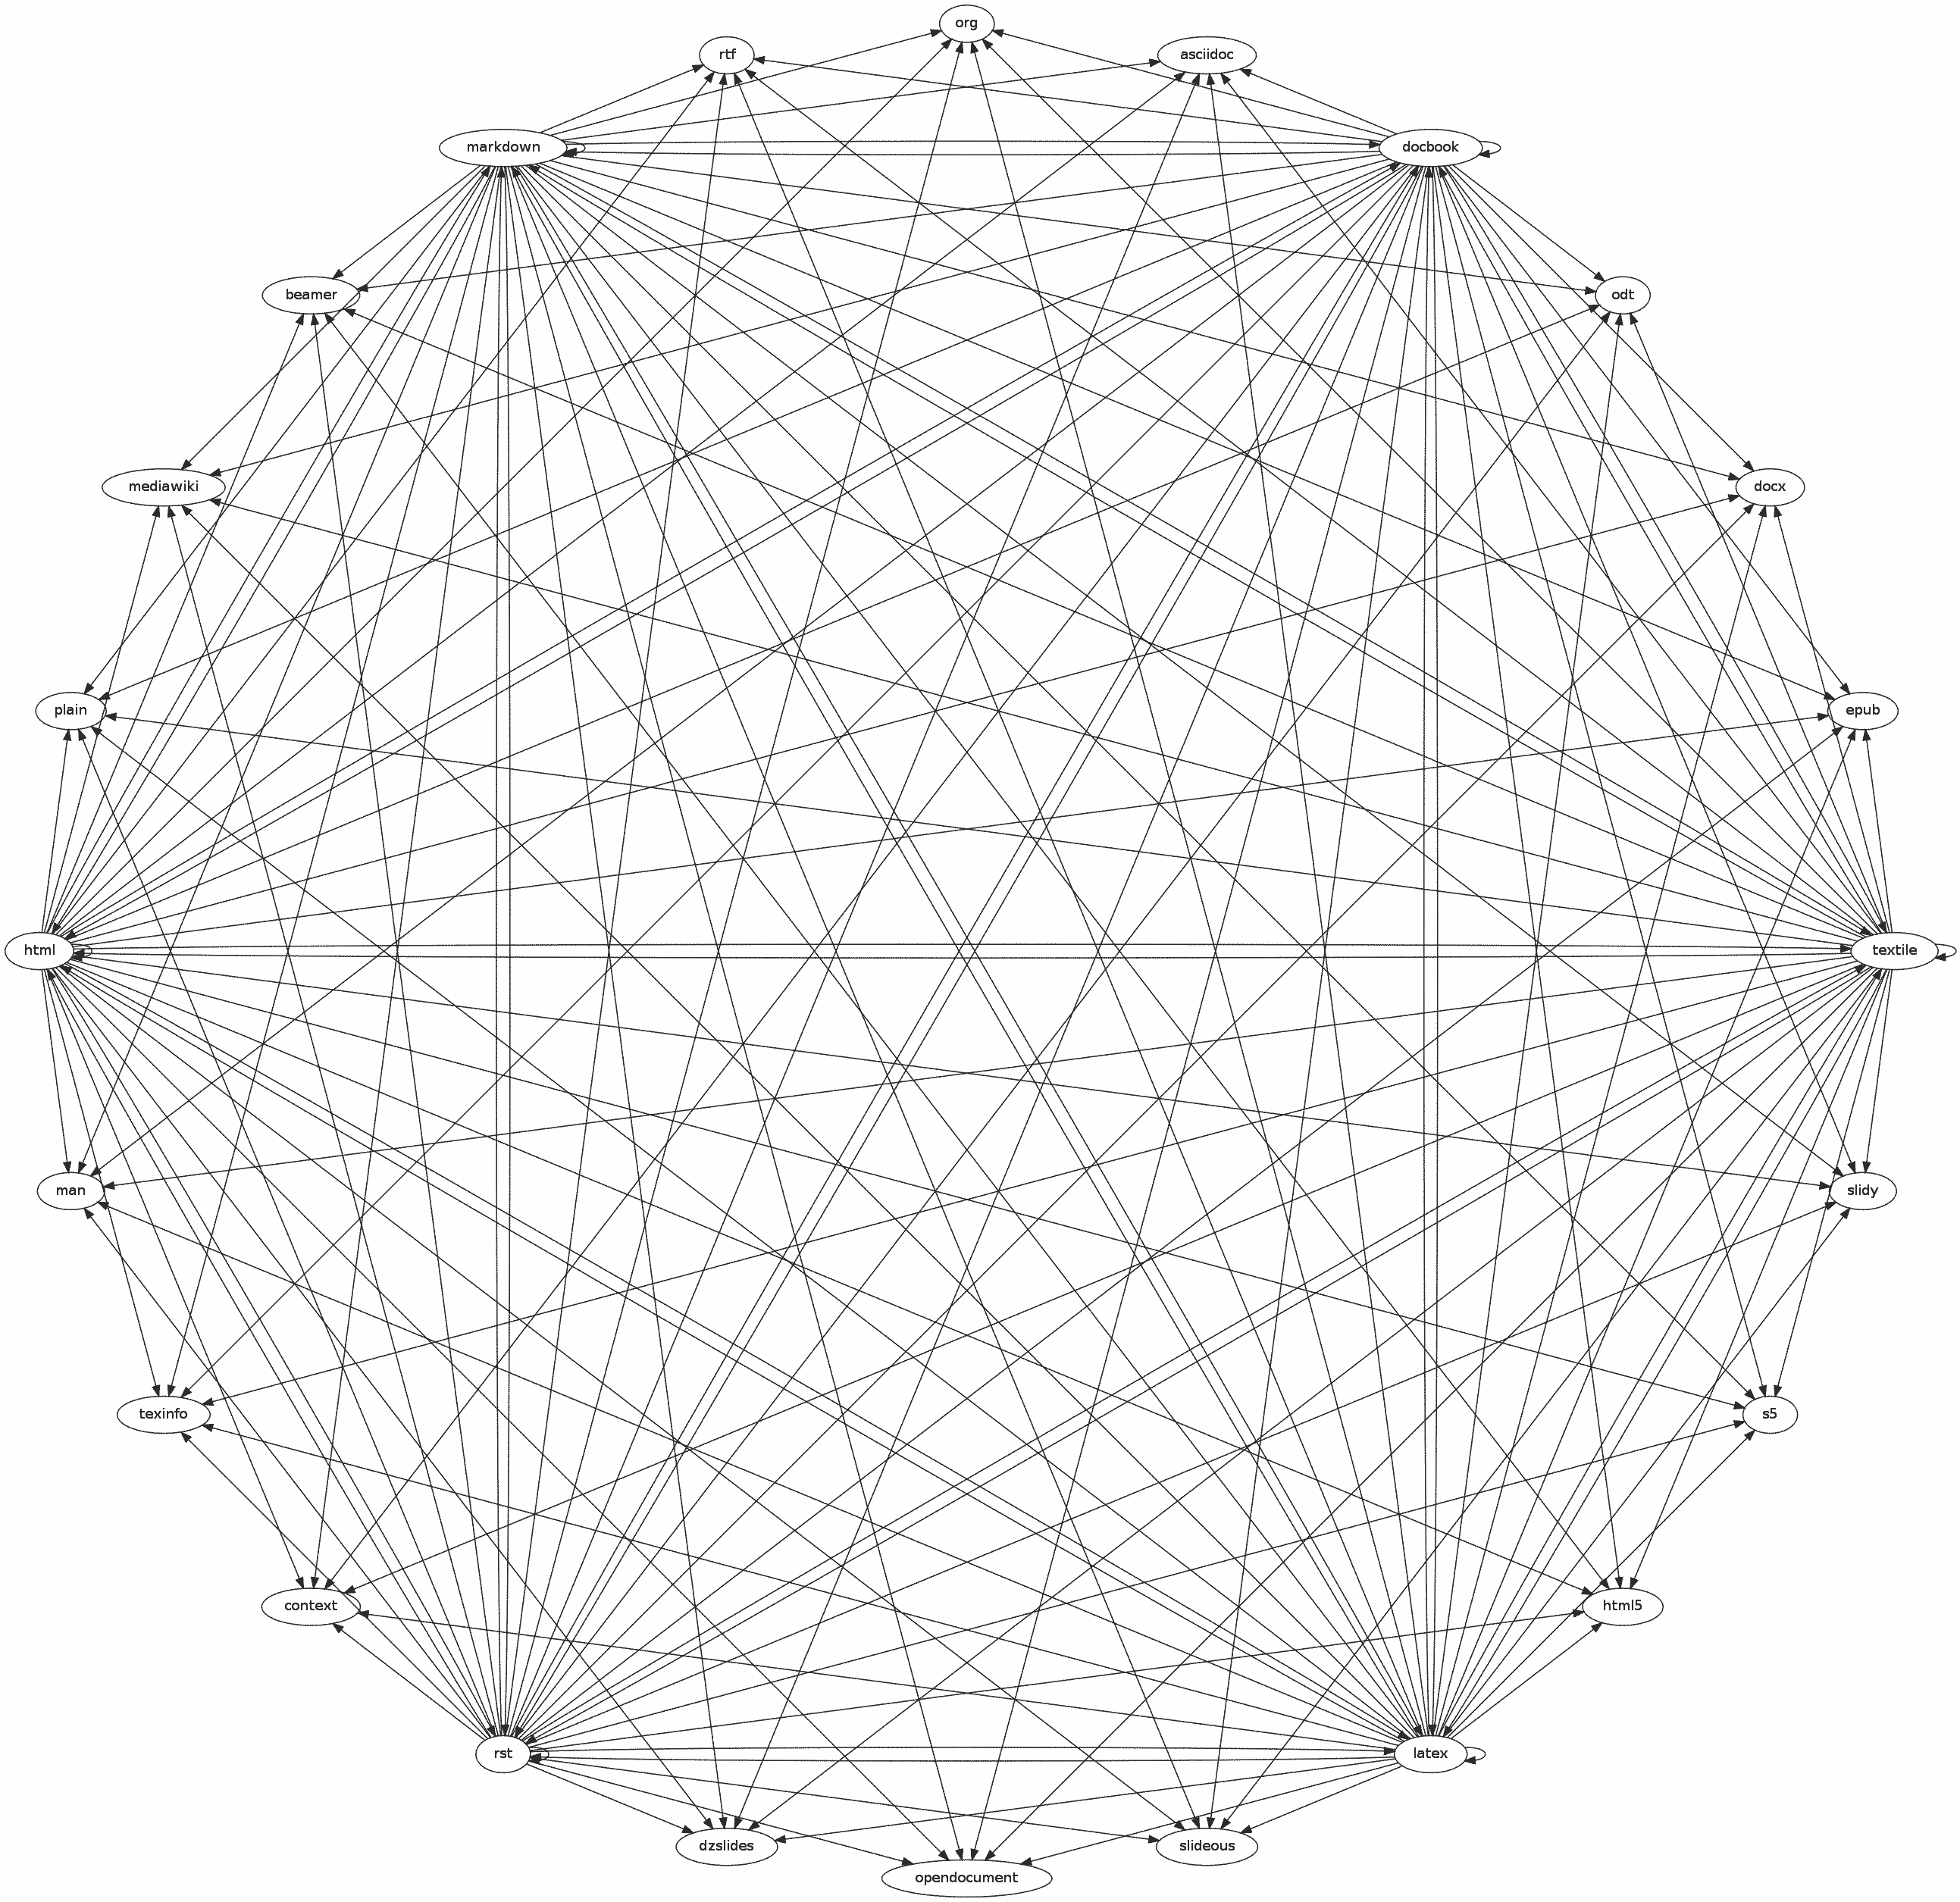
\includegraphics{./rez/diagram.png}
\caption{Pandoc Format Conversions}
\end{figure}

Again: Image copyright John MacFarlane

\end{document}
